\documentclass[tikz,border=10pt]{standalone}
\usepackage{amsmath}
\begin{document}

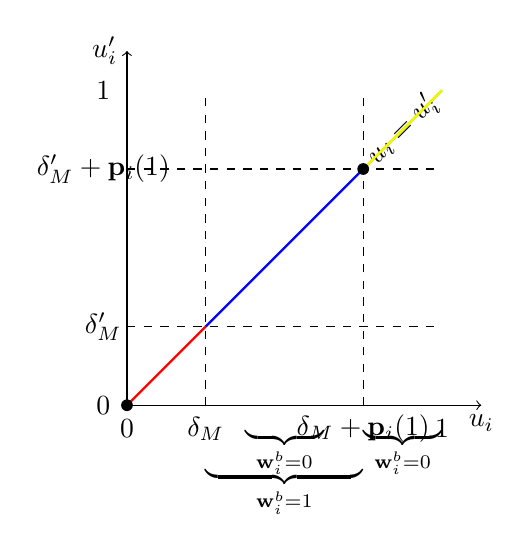
\begin{tikzpicture}
    % Axis
    \draw[->] (0,0) -- (4.5,0) node[below] {$u_i$};
    \draw[->] (0,0) -- (0,4.5) node[left] {$u'_i$};
    
    % Dashed lines
    \draw[dashed] (1,0) -- (1,4);
    \draw[dashed] (3,0) -- (3,4);
    \draw[dashed] (0,1) -- (4,1);
    \draw[dashed] (0,3) -- (4,3);
    
    % Colored segments
    \draw[red, thick] (0,0) -- (1,1);
    \draw[blue, thick] (1,1) -- (3,3);
    \draw[green, thick] (3,3) -- (4,4);
    
    % Labels
    \node at (0,-0.3) {$0$};
    \node at (1,-0.3) {$\delta_M$};
    \node at (3,-0.3) {$\delta_M + \mathbf{p}_i(1)$};
    \node at (4,-0.3) {$1$};
    \node at (-0.3,0) {$0$};
    \node at (-0.3,1) {$\delta'_M$};
    \node at (-0.3,3) {$\delta'_M + \mathbf{p}_i(1)$};
    \node at (-0.3,4) {$1$};
    
    \node at (2,-0.6) {$\underbrace{\hspace{1cm}}_{\mathbf{w}_i^b = 0}$};
    \node at (2,-1.1) {$\underbrace{\hspace{2cm}}_{\mathbf{w}_i^b = 1}$};
    \node at (3.5,-0.6) {$\underbrace{\hspace{1cm}}_{\mathbf{w}_i^b = 0}$};
    
    % Diagonal label
    \node[rotate=45] at (3.5,3.5) {$u_i = u'_i$};
    
    % Colored segment
    \draw[yellow, thick] (3,3) -- (4,4);

    % Node for delta_M + p_i(1)
    \node at (3,3) [circle,fill,inner sep=1.5pt]{};
    \node at (0,0) [circle,fill,inner sep=1.5pt]{};

\end{tikzpicture}

\end{document}